%!TEX root = adaptive_dict_kaf.tex

\section{A Probabilistic View of Kernel Adaptive Filters} % (fold)
\label{sec:a_novel_kernel_adaptive_filter}

Recall that standard KAF methods approximate the optimal weight element $W_i$ in eq. \eqref{eq:weights} by a subset of feature transformations of the observations. Yet simple, this is approach is rudimentary when compared to other sparsification procedures (see e.g. sparse GPs \cite{quinonero2005unifying}, where the centres are referred to as \emph{inducing points}). In fact, it is known that optimising over the centres/inducing points is more appropriate \cite{tobar_npk,zoubin_sparse}. Thus, we propose a probabilistic formulation of KAFs that allows for a principled choice of the dictionary, its initial weights, the kernel parameters and the noise variance.

\subsection{Generative Model}
Rather than using a suboptimal approximation based on the Representer Theorem, we define the dictionary $\cD_i=\{\s_j\}_{1:N_i}$, as well as the weights $\{\alpha_j\}_{1:N_i}$ and the remaining  hyperparameters in a probabilistic manner. This definition preserves the original formula of the KAF estimator with an added observation noise term, that is, 

%After this, the formula of the proposed estimator is still 
\begin{equation}
y_i = \sum_{j=1}^{N_i} \alpha_j K_{\sigma_k}(\x_i, \s_j) + \epsilon_i
\label{estimator}
\end{equation}
where $\epsilon_i\sim\cN(0,\sigma_\epsilon^2)$, $K_{\sigma_k}$ is a kernel with parameter $\sigma_k$, and we denote the input at time $i$ as $\x_i = [y_{i-d},\ldots, y_{i-1}]$, choosing a model order equal to $d$ without loss of generality. We emphasise that all the quantities are random variables and not chosen from heuristics as in the standard KAF setting, in particular, the dictionary $\cD=\{\s_1,\ldots,\s_{N_i}\}$ is not necessarily a subset of the observed inputs $\x_i,\ i\in\N$. We now focus on fixed dictionaries and have denoted $\cD_i=\cD$.

For an observed trajectory $Y=\{y_1,\ldots, y_N\}$ the model likelihood can be written in product form, since the process $y_i,\ i\in\N$, is $d$-order Markovian and admits the decomposition
\begin{equation}
\begin{split}
    p(Y) &= \prod_{i=d}^{N} p(y_i\vert \x_i) \\ &= \prod_{i=d}^{N} \frac{1}{\sqrt{2\pi\sigma_\epsilon^2}}\exp\left( -\frac{\left(y_i - \balpha^\top K_{\sigma_k}(\x_i, \cD)\right)^2 }{2\sigma_\epsilon^2}\right) 
\end{split}
\end{equation}
where $\balpha_i=[\alpha_1,\cdots,\alpha_{N_i}]^\top$ is the vector of filter weights at time $i$, and $K_{\sigma_k}(\x_i, \cD)$ denotes the vector of kernel evaluations of the input $\x_{i}$ and each element of the dictionary $\cD$. Furthermore, we can place priors on the weight vector $\balpha_i$, the kernel parameter $\sigma_{k}$ and the noise variance $\sigma_\epsilon$:
%allows measure the variability
\begin{align*}
    p(\balpha) &= \frac{1}{\sqrt{2 \pi l_\alpha^2}}\exp\left( -\frac{\left\| \balpha \right\|^2}{2 l_\alpha^2}  \right)
    \label{eq:coef_prior}\\
   	p(\sigma_{k}) & = \mathcal{N}_{\mathbb{R}^+}(0,v_k)\\ %\red{(\ not\ defined)}\\
	p(\sigma_{\epsilon}) & = \mathcal{N}_{\mathbb{R}^+}(0,v_\epsilon)
\end{align*}
where $p(\balpha)$ enforces small and regular filter weights, and the half-Normal priors on both the kernel parameter $\sigma_k$ and the noise variance $\sigma_\epsilon$ ensure positive and close-to-zero values. 

We propose to use the following prior for the dictionary
\begin{equation}
	 p(\cD) = \frac{1}{\sqrt{2 \pi l_\cD^2}}\exp\left( -\frac{\left\|K_\sigma(\cD,\cD) \right\|^2}{2 l_\cD^2}  \right)
	\label{eq:dict_prior}
\end{equation}
this is an exponential distribution on the square norm of the Gram matrix evaluated on the dictionary. Consequently, this prior produces dictionaries for which $\left\|K_\sigma(\cD,\cD) \right\|^2$ is close to zero. For a Gaussian kernel, this implies that the samples of the dictionary will be far from one another, since $\left\|K_\sigma(\cD,\cD) \right\|^2 = \sum_{j,k=1}^{N_i}K^2_{\sigma_k}(\s_j,\s_k)$. Therefore, $p(\cD)$ in eq. \eqref{eq:dict_prior} is a sparsity-inducing prior that avoids redundancy arising from choosing the centres directly from data, as it is the case in the coherence \cite{richard09} or novelty \cite{platt91} sparsification criteria. Furthermore, we place half-Normal hyperpriors on $l_\alpha$ and $l_\cD$, with zero mean an variances $v_{\balpha}$ and $v_{\cD}$ respectively.


%The reason we considered the norm of the Gram matrix is as a sparsity metric is that the kernel  is already being used as a similarity function among measurements within KAF. For the Gaussian kernel this similarity degree spans from $0$, which states completely different data based on the kernel width, to $1$, meaning comparison over the same datum. Then, a desirable Gram matrix is one closer to an identity form, thus having a minimal norm given a fixed number of centers.



%posterior:
%\begin{equation}
%    p(D) = \prod_{t=1}^{N} -\frac{1}{\sqrt{2\pi\sigma_\epsilon^2}}\exp\left( -\frac{\left(y_t - \sum_{x_i\in D} \alpha_i K(x, x_i)\right)^2 }{2\sigma_\epsilon^2}\right)  \frac{1}{2 \pi l^2}\exp\left( -\frac{\left\|k_\sigma(D_t,D_t) \right\|^2}{2 l^2}  \right)
%\end{equation}
\iffalse
\begin{equation}
\begin{split}
	\log p(\cD | Y) =  - \frac{1}{2}\bigg(\log \frac{v_{k}^{2} \pi}{2} + \log \frac{v_{e}^{2} \pi}{2} + \log \frac{v_{\cD}^{2} \pi}{2} + \log \frac{v_{\balpha}^{2} \pi}{2} \\ 
	N\log 2 \pi  \sigma^2_\epsilon + \log 2 \pi l_\cD^2 + \log 2 \pi l_\balpha^2
	- \frac{\sigma_{k}^{2}}{ v_{k}^{2}} - \frac{\sigma_{\epsilon}^{2}}{ v_{\epsilon}^{2}}	 - \frac{l_{\balpha}^{2}}{ v_{\balpha}^{2}} - \frac{l_{\cD}^{2}}{ v_{\cD}^{2}}\bigg)\\
	+ \frac{-\sum_{i=1}^{N} \left(y_i - \balpha^\top K_{\sigma_k}(\x_i, \cD)\right)^2}{2\sigma_\epsilon^2} -\frac{\left\|K_\sigma(\cD,\cD) \right\|^2}{2 l_\cD^2} -\frac{\left\|\balpha \right\|^2}{2 l_\balpha^2}
\end{split}
\label{eq:log-posterior}
\end{equation}
%\red{aqui falta el prior sobre $\sigma_k$ ? }
and will use it for finding appropriate parameters in the next section.
\fi

Although the full posterior can be calculated analytically (up to a normalising constant), we do not show it here due to space constraints. However, observe that besides the regularisation terms, the three main terms of the log-posterior are
\begin{equation*}
\begin{split}
  \frac{-\sum_{i=1}^{N} \left(y_i - \balpha^\top K_{\sigma_k}(\x_i, \cD)\right)^2}{2\sigma_\epsilon^2} -\frac{\left\|K_\sigma(\cD,\cD) \right\|^2}{2 l_\cD^2} -\frac{\left\|\balpha \right\|^2}{2 l_\balpha^2}.
\end{split}
\label{eq:log-posterior}
\end{equation*}
Therefore, optimisation of the log-posterior of the proposed model is a trade-off among data fit (first term), sparsity of the dictionary (second term) and regular weights (third term). 


\subsection{Offline optimisation of the log-posterior}
 

%To do so, we used the library PyMC3 \cite{salvatier2016probabilistic} is used, which includes tools for defining log-posterior functionals; perform MAP estimation through gradient-based methods like BFGS\cite{fletcher2013practical}; and/or sample from the posterior using MCMC algorithms such as Metropolis-Hastings\cite{hastings1970monte}. In this case, we use BFGS to have an initial condition on the Markov chain simulation, and sometimes consider it as direct optimal, if the simulation shows that the initial MAP of the parameters has started at the chain stationary distribution.

%We can use this to perform what we will call as offline estimation, where we take an initial training subset from the signal to tune its parameters through the optimisation schema presented previously, and then perform estimation over the rest of the signal using Eq. \eqref{estimator} with the optimised parameters. To accomplish this, the only parameters needed to be set previously are the number of elements in the dictionary (not to be confused with the elements themselves) and the filter order (delay of the inputs for the autorregresive model). 

To illustrate the suitability of the proposed approach to find appropriate parameters, we present the following synthetic-data example. We generated 1000 observations of the first channel of the Lorenz Chaotic Attractor \cite{lorenz1963deterministic} and implemented a kernel estimator as that in eq. \eqref{estimator}, with dictionary of size 5 and order $d=5$. We considered different subsets for training and then predicted the remaining part of the time series with the (fixed) parameters learned according to the model in eq. \eqref{estimator}. The motivation for this experiment is to assess how the predictive ability of the  model improves as more data are seen. 

Fig. \ref{fig:lorenz-series} shows the prediction of the model trained using 35 (top), 60 (middle) and 250  (bottom) samples, where the chosen parameters were set to the mean of the sample posterior approximated using Markov chain Monte Carlo (MCMC). Notice how the estimation improves pointwise, reaching all the extrema of the signal for the 250-training-sample case, even though this is a non-adaptive model. Fig. \ref{fig:lorenz-gram} shows the Gram matrix for the optimal centres for the case of 250 training samples, just as expected, sampling from eq. \eqref{eq:dict_prior} delivers a sparse dictionary characterised by a close-to-diagonal Gram matrix.

\begin{figure}[t!]
	\centering
	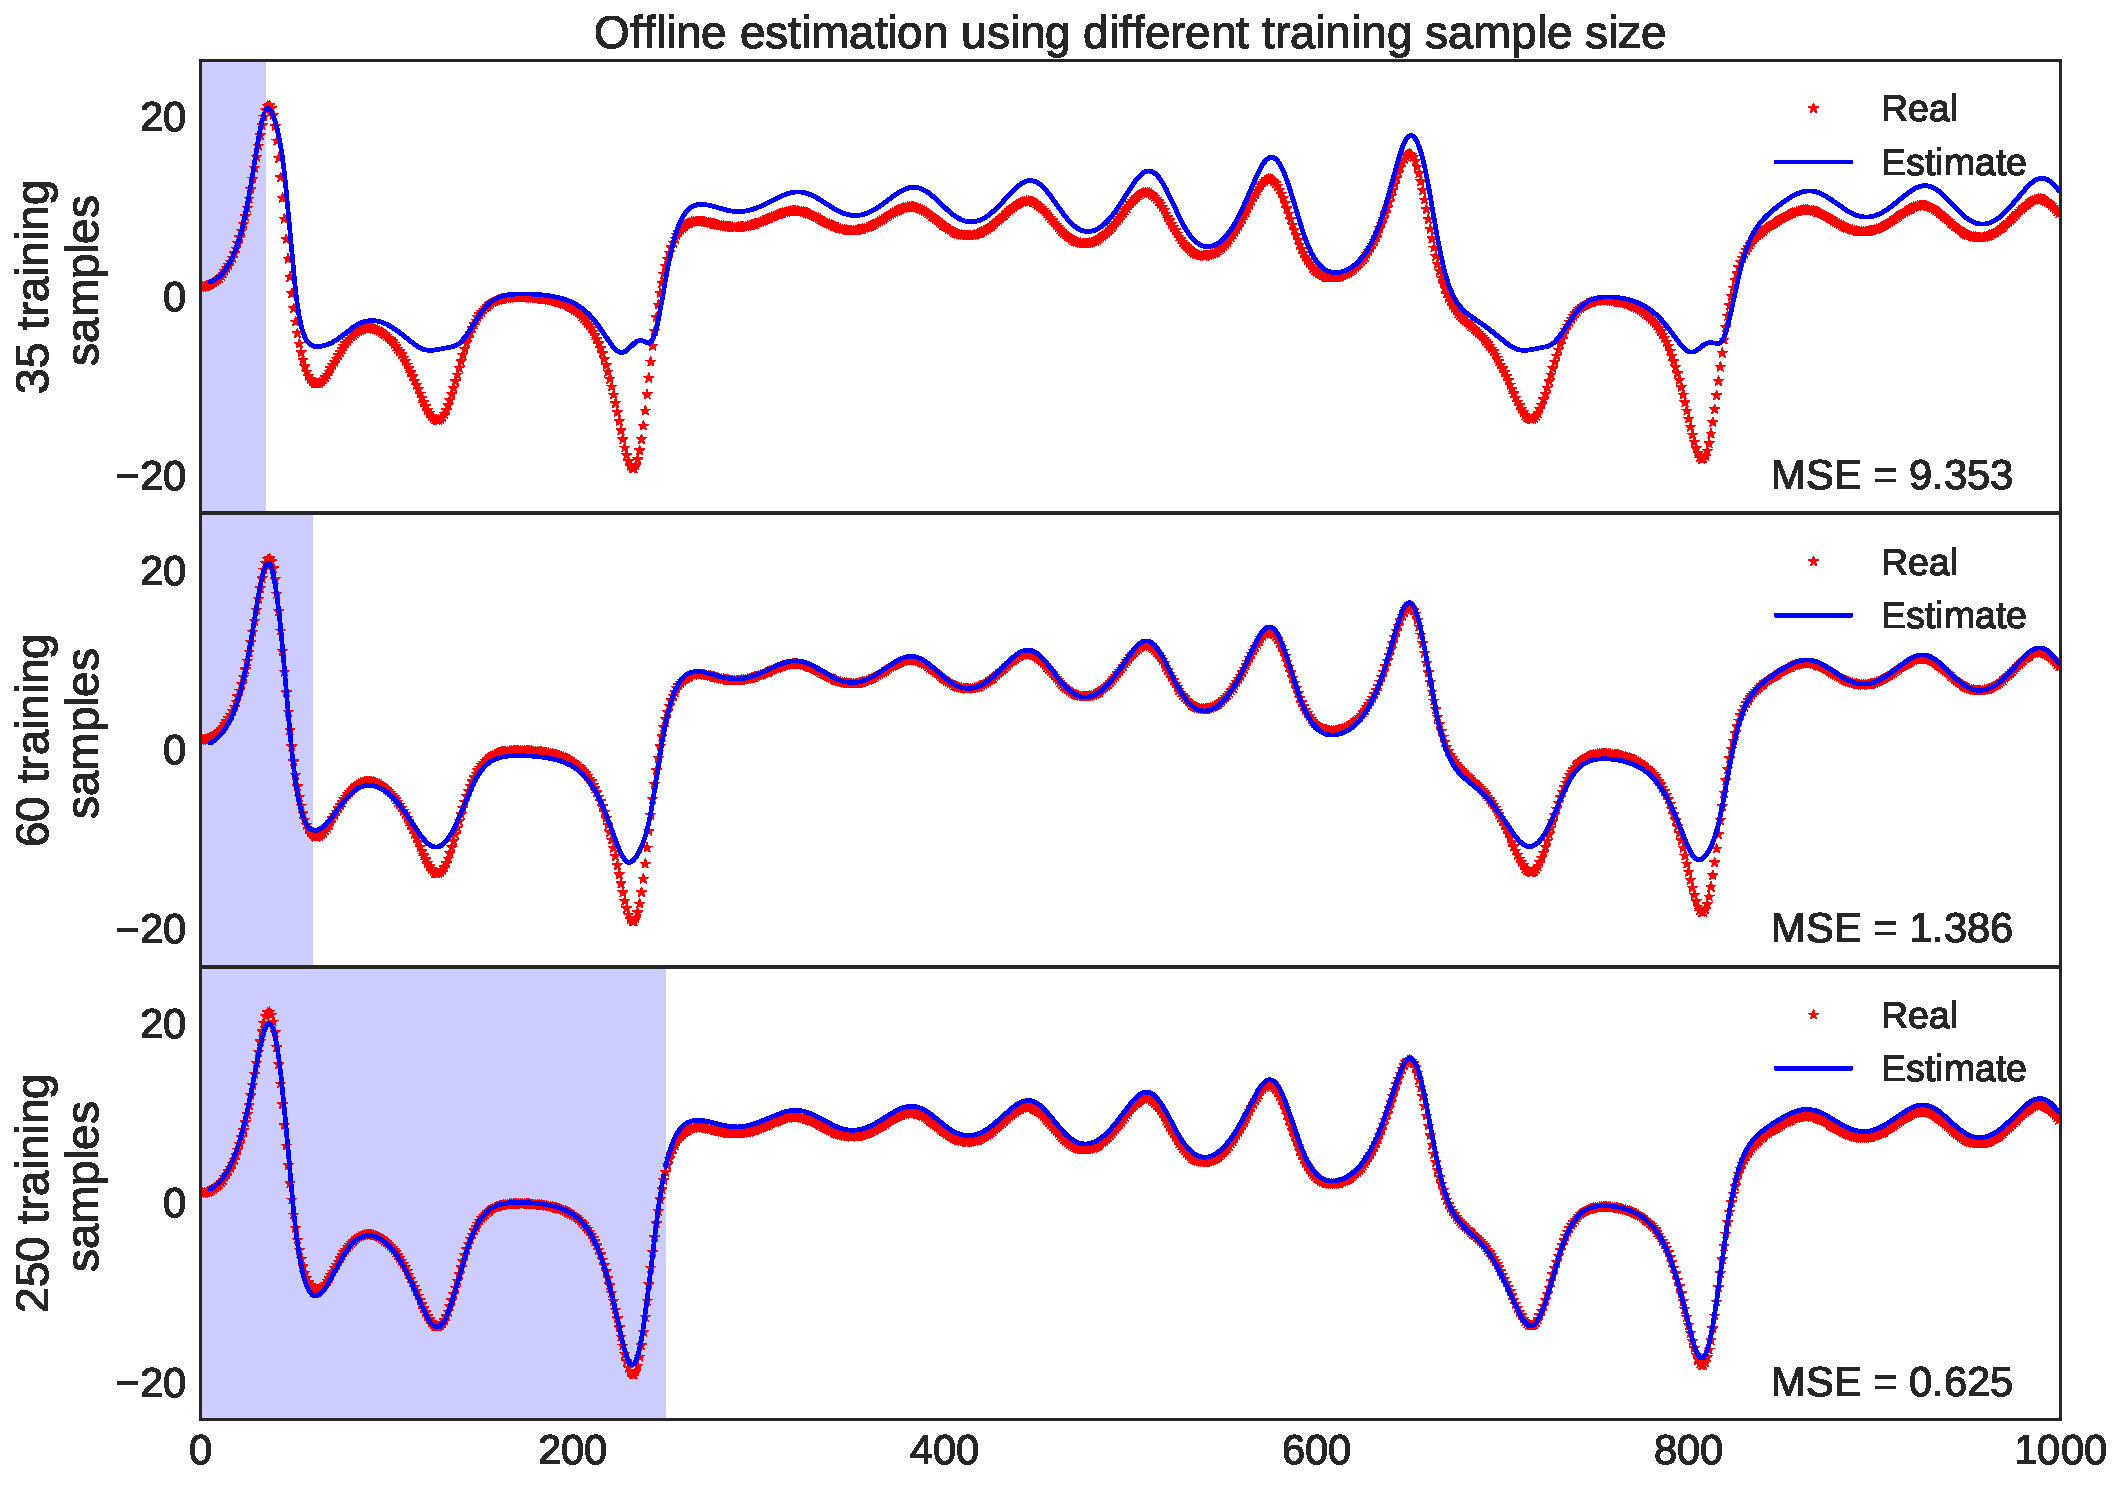
\includegraphics[width=0.5\textwidth]{img/Lorenz_Offline3}
	\caption{Prediction of the Lorenz series using the model in eq. \eqref{estimator} with fixed parameters trained with different subsets of data. The blue area indicates the training data in each case.}
	\label{fig:lorenz-series}
\end{figure}

\begin{figure}[t!]
	\centering
	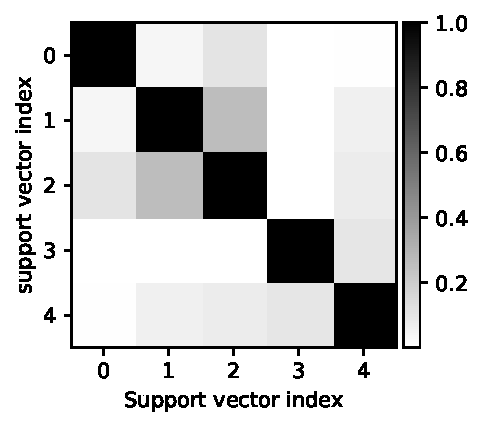
\includegraphics[width=0.2\textwidth]{img/Gram_lorenz}
	\caption{Gram matrix of size $5$ for the $250$ sample training case.}
	\label{fig:lorenz-gram}
\end{figure}

